\documentclass[12pt]{article}
%Gummi|065|=)
\usepackage{amsmath, amsfonts, amssymb}
\usepackage[margin=0.5in]{geometry}
\usepackage{xcolor}
%\usepackage{graphicx}
%\usepackage{graphicx}
\newcommand{\off}[1]{}
\DeclareMathSizes{20}{30}{21}{18}

\newcommand{\myhrule}{}

\newcommand{\dash}{
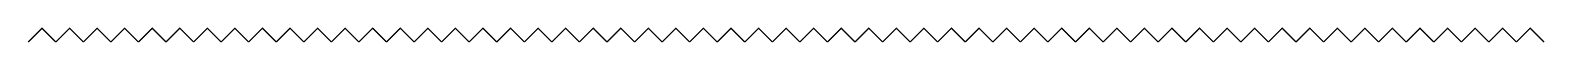
\begin{tikzpicture}[scale=0.35]
\foreach \x in {1,...,55}{
	\draw (\x,-0.25)--(\x+0.5,0.25)--(\x+1,-0.25);
}
\end{tikzpicture}
}

\usepackage{tikz}

\title{\textbf{ Examples: Sachdev-Ye-Kitaev}}
\author{John D Mangual}
\date{}
\begin{document}

\fontfamily{qag}\selectfont \fontsize{25}{30}\selectfont

\maketitle

\fontfamily{qag}\selectfont \fontsize{12}{10}\selectfont

\noindent The point of this article is to make heads or tails of the Sachdev-Ye-Kitaev model.  They made it look interesting in the video and I hope it can be the case.  

\newpage

\fontfamily{qag}\selectfont \fontsize{12}{10}\selectfont

\begin{thebibliography}{}

\item Joseph Polchinski, Vladimir Rosenhaus \textbf{The Spectrum in the Sachdev-Ye-Kitaev Model} \texttt{arXiv:1601.06768}

\item Juan Maldacena, Douglas Stanford \textbf{Comments on the Sachdev-Ye-Kitaev Model} \texttt{arXiv:1604.07818}

\end{thebibliography}



\end{document}